\documentclass[pdftex]{article}
\usepackage{times}
\usepackage{amsmath}
\usepackage{amsfonts}
\usepackage{fancyhdr}
\usepackage{amssymb}
\usepackage{verbatim}
\usepackage{graphicx}
\usepackage{float}
\usepackage{multicol}
\usepackage[section]{placeins}
\usepackage[margin=1.0in]{geometry}
\usepackage[numbered=true]{bookmark}

\begin{document}

\fancyhead[L]{PRELIMINARY}
\fancyfoot[L]{Revision: 0.1/PRELIMINARY}
\pagestyle{fancy}

\title{RED TIN Internal Logic Analyzer Datasheet\\Revision 0.1}
\author{Andrew D. Zonenberg\\
	\texttt{azonenberg@drawersteak.com}}
\date{\today}
\maketitle

\paragraph*{}
{\bf NOTE: } This document is preliminary and is subject to change. The software/firmware described in this document is
an alpha release which may contain bugs or errata. While a best effort attempt has been made to list all known errata
in this document, comprehensive testing has not yet been completed.

\paragraph*{}
Bug reports are welcomed. Please email reports to the email address listed on this title page.

\pagebreak
\tableofcontents
\pagebreak

\pagebreak
\section{Introduction} 

\paragraph*{}
RED TIN is an internal logic analyzer for debugging FPGA designs. It consists of three components - the capture module,
the interface wrapper, and the user interface. The first two are Verilog modules that run on the DUT FPGA and the last
is a C++ GUI application.

\paragraph*{}
RedTinLogicAnalyzer, the {\bf capture module}, is responsible for sampling data from the DUT and storing it to a
N-sample circular buffer. When waiting for a trigger event the buffer is continually rotating and data is written to the
Mth position in the buffer. Once triggered the start and stop pointers are frozen and data is stored until the end of
the buffer is reached. This results in M samples before the trigger and (N-M) after. Currently N and M have values of
512 and 16, respectively. In a future release the depth N will likely be parameterizable, and the the value of M will be
adjustable at run time between captures.

\paragraph*{}
The {\bf interface wrapper} is responsible for bridging communications from the capture module to a PC. The interface
may be anything supported by the target board; currently only a UART at 500kbaud is implemented (RedTinUARTWrapper).
Future releases may add support for other interfaces such as JTAG, Ethernet, USB.

\paragraph*{}
The {\bf user interface} allows the user to specify the signals and trigger parameters to be used by the system. Once
a capture has completed, the UI reformats the raw binary data dump into a standard .vcd file and displays it in a
third-party waveform viewer. This is currently gtkwave (hard coded) however support for additional viewers will be
added in a future release.

\paragraph*{}
The Verilog components have only been tested on a Xilinx Spartan-6 FPGA, but were written in a portable fashion and
should be usable with any Verilog toolchain. Reports of successful or failed tests on other platforms are welcome.

\paragraph*{}
The UI application was written in C++ using the gtkmm GUI framework and should be easy to port to other platforms
however the alpha release has only been tested on 64-bit Debian ``Squeeze". The UART communications code is currently
not as modular as desirable; a future refactoring will make it easier to add suport for new bridges or interface APIs.
Reports of successful or failed tests on other platforms are welcome.

\paragraph*{}
The name ``RED TIN" has no meaning whatsoever. It was chosen by the following algorithm (used when nobody involved can
think of something that sounds good):
\begin{verbatim}
do
{
  a = random adjective
  n = random noun
} while(!sounds_good(a + " " + n))
\end{verbatim}

\pagebreak
\section{Capture module usage}


\pagebreak
\section{User interface operation}

\paragraph*{}
\begin{figure}[h]
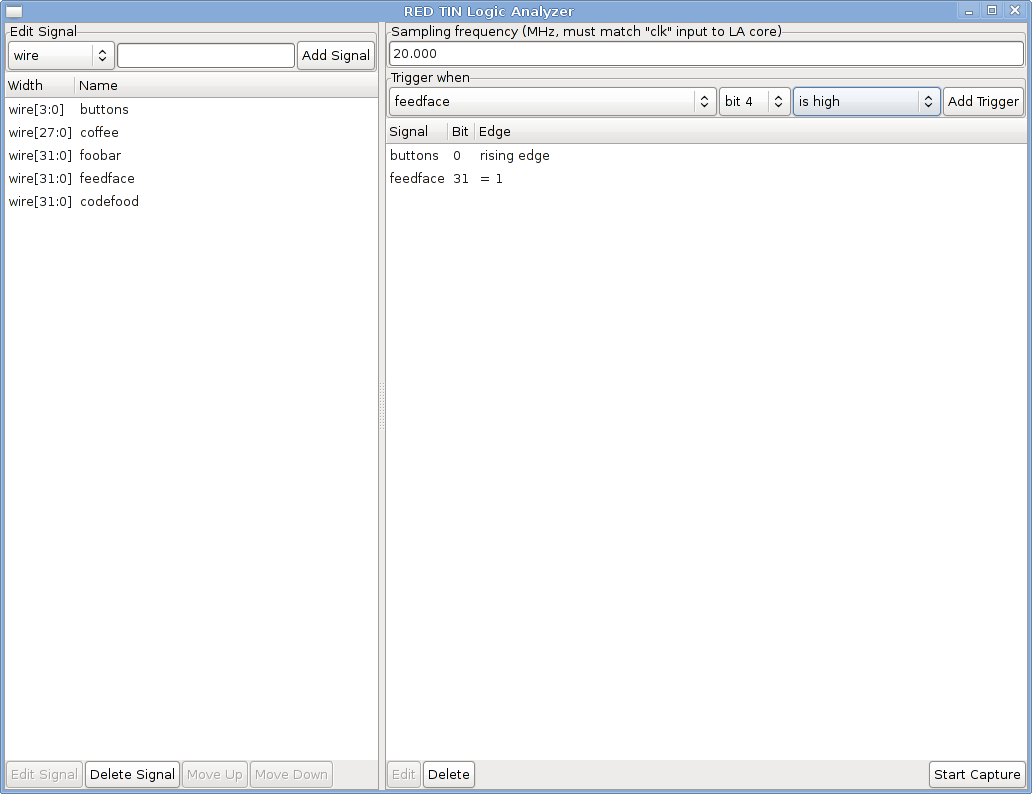
\includegraphics[scale=0.45]{gui-shot1.png}
\caption{Screenshot of UI}
\label{gui-overview}
\end{figure}

\pagebreak
\section{Errata}

\paragraph*{}
All known bugs were fixed before the alpha release. If I missed any please file a report and let me know!

\end{document}
